% ==================================================================
%  midterm.tex  —  Revised version (fixed \hyp{} usage)
% ==================================================================
\documentclass[svgnames]{article}

% -------------------------------------------------------------
%  Packages
% -------------------------------------------------------------
\usepackage{graphicx}

% -- mathematics ------------------------------------------------
\usepackage{amssymb}
\usepackage{amsmath}
\usepackage{esint}
\usepackage{geometry}
\usepackage{hyphenat}          % \hyp{} for breakable hyphens

% -- figures / floats ------------------------------------------
\usepackage{float}
\usepackage{caption}

% -- listings and code -----------------------------------------
\usepackage{listings}

% -- tikz / pgfplots -------------------------------------------
\usepackage{pgfplots}
\pgfplotsset{compat=1.15}
\usepackage[most]{tcolorbox}

% custom coloured box for highlights
\newtcolorbox{mybox}{
    enhanced,
    boxrule=0pt,frame hidden,
    colback=green!10!white,
    sharp corners
}

% -------------------------------------------------------------
%  Document metadata
% -------------------------------------------------------------
\title{Midterm \textendash{} Simulating Electrically Detected Magnetic Resonance}
\author{Deval Deliwala}

% -------------------------------------------------------------
\begin{document}
\maketitle

% =============================================================
\section{Abstract}
% =============================================================
Understanding the microscopic spin processes that underpin Electrically Detected Magnetic Resonance (EDMR) is essential for refining both experimental protocols and device design. In this work we present a complete, parameterised description of \emph{spin\hyp{}dependent recombination} (SDR) in a \mbox{two\hyp{}electron}, \mbox{two\hyp{}nucleus} defect complex representative of divacancies in 4H\,\textendash{}SiC. By fitting the resulting SDR model to combined \mbox{near\hyp{}zero\hyp{}field} and \mbox{resonance\hyp{}mode} EDMR data, we extract the hyperfine tensors, \mbox{zero\hyp{}field\hyp{}splitting} parameters, and exchange coupling that govern the defect. To the best of our knowledge this is the first demonstration of a \mbox{sweep\hyp{}wide}, fully \mbox{self\hyp{}consistent} SDR simulation for EDMR.

% =============================================================
\section{Introduction}
% =============================================================
Electron Spin Resonance (ESR) traditionally detects \mbox{microwave\hyp{}induced} transitions inductively, which limits its sensitivity when the number of participating spins is small. EDMR circumvents this limitation by probing changes in an \emph{electrical} observable—usually a source–drain or photocurrent—while the sample is exposed to resonant microwave radiation in a static magnetic field~$B$. Because the detected signal is proportional to the device current, the technique can be implemented on finished semiconductor structures under realistic biasing conditions and routinely achieves sensitivities down to a few hundred spins.

The key physical ingredient is \emph{spin\hyp{}dependent recombination}. Consider a \mbox{conduction\hyp{}band} electron captured by a deep paramagnetic centre and subsequently paired with a localised hole. The intermediate electron–hole pair may exist in either a singlet state $|S\rangle$ or one of three triplet states $|T_{+}\rangle$, $|T_{0}\rangle$, $|T_{-}\rangle$. Only the singlet configuration couples efficiently to the lattice, enabling radiative or \mbox{non\hyp{}radiative} recombination that removes the charge carriers from the band and thereby reduces the measured current. Triplet pairs, by contrast, are long\hyp{}lived and tend to re\hyp{}inject carriers back into the conduction band. Resonant microwave irradiation flips one of the electron spins, converts triplet population into singlet population, and thus modulates the current. Recording the current change $\Delta I(B)$ as a function of $B$ yields an EDMR spectrum that encodes the defect $g$\,\textendash{}tensor, hyperfine couplings, and any \mbox{crystal\hyp{}field} interactions. Consequently EDMR has become a central characterisation tool for interface traps, dopants, and nascent \mbox{spin\hyp{}qubit} platforms.

% =============================================================
\section{The Spin Hamiltonian}\label{sec:spin_ham}
% =============================================================
The total Hamiltonian of the defect system combines four well\hyp{}defined interactions:
\[
  \hat{H}_0 = \hat{H}_{Z} + \hat{H}_{\mathrm{HF}} + \hat{H}_{\mathrm{ZFS}} + \hat{H}_{\mathrm{EX}}.
\]
Each term is summarised below; full derivations and the associated \verb|Python| source code can be found in our online manuscripts.\footnote{https://dev-undergrad.dev/posts/spin\_hamiltonian\_derivation/}\footnote{https://dev-undergrad.dev/posts/spin\_hamiltonian\_code/}

\paragraph{Zeeman interaction.} In the coupled\hyp{}spin basis $\{|s,m\rangle\}$, where $s\in\{0,1\}$ denotes the total electron spin and $m$ its projection onto $\hat{z}$, the Zeeman term reads
\[
  \hat{H}_{Z}\,|s,m\rangle = m\,g\,\mu_{\mathrm B} B\;|s,m\rangle.
\]
Here $g$ is the isotropic electron $g$\,\textendash{}factor and $\mu_{\mathrm B}$ the Bohr magneton.

\paragraph{Zero\hyp{}field splitting (ZFS).} Axial ($D$) and rhombic ($E$) \mbox{crystal\hyp{}field} parameters lift the degeneracy of the $m$\,\textendash{}sub\hyp{}levels even at $B=0$:
\begin{align}
 \hat{H}_{\mathrm{ZFS}}\,|s,m\rangle &= D m^2 |s,m\rangle - \frac{D}{3}s(s+1)|s,m\rangle\\[3pt]
 &\quad+\frac{E}{2}\bigl[s(s+1)-m(m+1)\bigr]|s,m+2\rangle\\[3pt]
 &\quad+\frac{E}{2}\bigl[s(s+1)-m(m-1)\bigr]|s,m-2\rangle.
\end{align}
If $E=0$ the Hamiltonian remains diagonal in $m$; otherwise the $m\,\to\,m\pm2$ terms mix sub\hyp{}levels of identical spin multiplicity.

\paragraph{Exchange interaction.} When two unpaired electrons reside on adjacent sites, the Heisenberg exchange coupling $J$ splits the singlet and triplet manifolds:
\[
  \hat{H}_{\mathrm{EX}}\,|s,m\rangle = -J\left[\frac{s(s+1)-\tfrac{3}{2}}{2}\right] |s,m\rangle.
\]

\paragraph{Hyperfine interaction.} For a pair of nuclear spins $I_1$ and $I_2$
(both $\tfrac12$), the secular and \mbox{non\hyp{}secular} contributions combine
into the operator given in Eq.~\eqref{hyperfine}. The resulting matrix has
dimension $16\times16$, corresponding to the product basis
$|m_a\,m_b\,m_{I_1}\,m_{I_2}\rangle$ with $m\in\{\uparrow,\downarrow\}$.

\begin{equation} \label{hyperfine}
    \begin{split}
    \hat{H}_{HF} |&m_a, m_b, m_{I_1}, m_{I_2}\rangle  \\
                       &= \hbar^2 \sum_{p=1}^{2} \left(A_{apz}m_am_{I_p} +
                       A_{bpz}m_bm_{I_p} \right) |m_a, m_b, m_{I_1},
                       m_{I_2}\rangle  \\ 
                       &+\frac{\hbar^2}{4}\left[\left( A_{a1x}-A_{a1y} \right)
                           \delta_{m_a, m_{I_1}} + \left( A_{a1x} + A_{a1y}
                           \right) \delta_{m_a, -m_{I_1}}  \right] |-m_a, m_b,
                           -m_{I_1}, m_{I_2}\rangle \\ 
                       &+\frac{\hbar^2}{4}\left[\left( A_{a2x}-A_{a2y} \right)
                           \delta_{m_a, m_{I_2}} + \left( A_{a2x} + A_{a2y}
                           \right) \delta_{m_a, -m_{I_2}}  \right] |-m_a, m_b,
                            m_{I_1}, -m_{I_2}\rangle \\ 
                       &+\frac{\hbar^2}{4}\left[\left( A_{b1x}-A_{b1y} \right)
                           \delta_{m_b, m_{I_1}} + \left( A_{b1x} + A_{b1y}
                           \right) \delta_{m_b, -m_{I_1}}  \right] |m_a, -m_b,
                           -m_{I_1}, m_{I_2}\rangle \\ 
                       &+\frac{\hbar^2}{4}\left[\left( A_{b2x}-A_{b2y} \right)
                           \delta_{m_b, m_{I_2}} + \left( A_{b2x} + A_{b2y}
                           \right) \delta_{m_b, -m_{I_2}}  \right] |m_a, -m_b,
                           m_{I_1}, -m_{I_2}\rangle.   
\end{split}
\end{equation}

\medskip
Collecting every contribution, we express the Hamiltonian symbolically parameterised by
\[
  \theta = \{A_{a1},A_{a2},A_{b1},A_{b2},g_e,g_{n1},g_{n2},\mu_{\mathrm B},\mu_{\mathrm N},B,D_1,D_2,J\}.
\]

% =============================================================
\section{Eigenenergy Simulations}\label{sec:eigensims}
% =============================================================
With $\hat{H}_0(\theta)$ in hand, we compute its eigenenergies $E_k(B)$ to identify crossings that feed into the EDMR spectrum. The numerical workflow is summarised in Listing~\ref{lst:workflow}; step~4 employs the Hungarian algorithm to track eigenvectors as $B$ varies, thereby suppressing artificial repulsion due to sorting ambiguities.

\begin{lstlisting}
1. For each magnetic field B:
2.     assemble H0(B) -> numeric 16x16 matrix
3.     call LAPACK 'geev' to get eigenvalues/vectors
4.     match eigenvectors to |s,m>|mI1>|mI2> basis via Hungarian algorithm
5. Plot eigenenergies E_k(B) for k = 1..16
\end{lstlisting}

\begin{figure}[H]
  \centering
  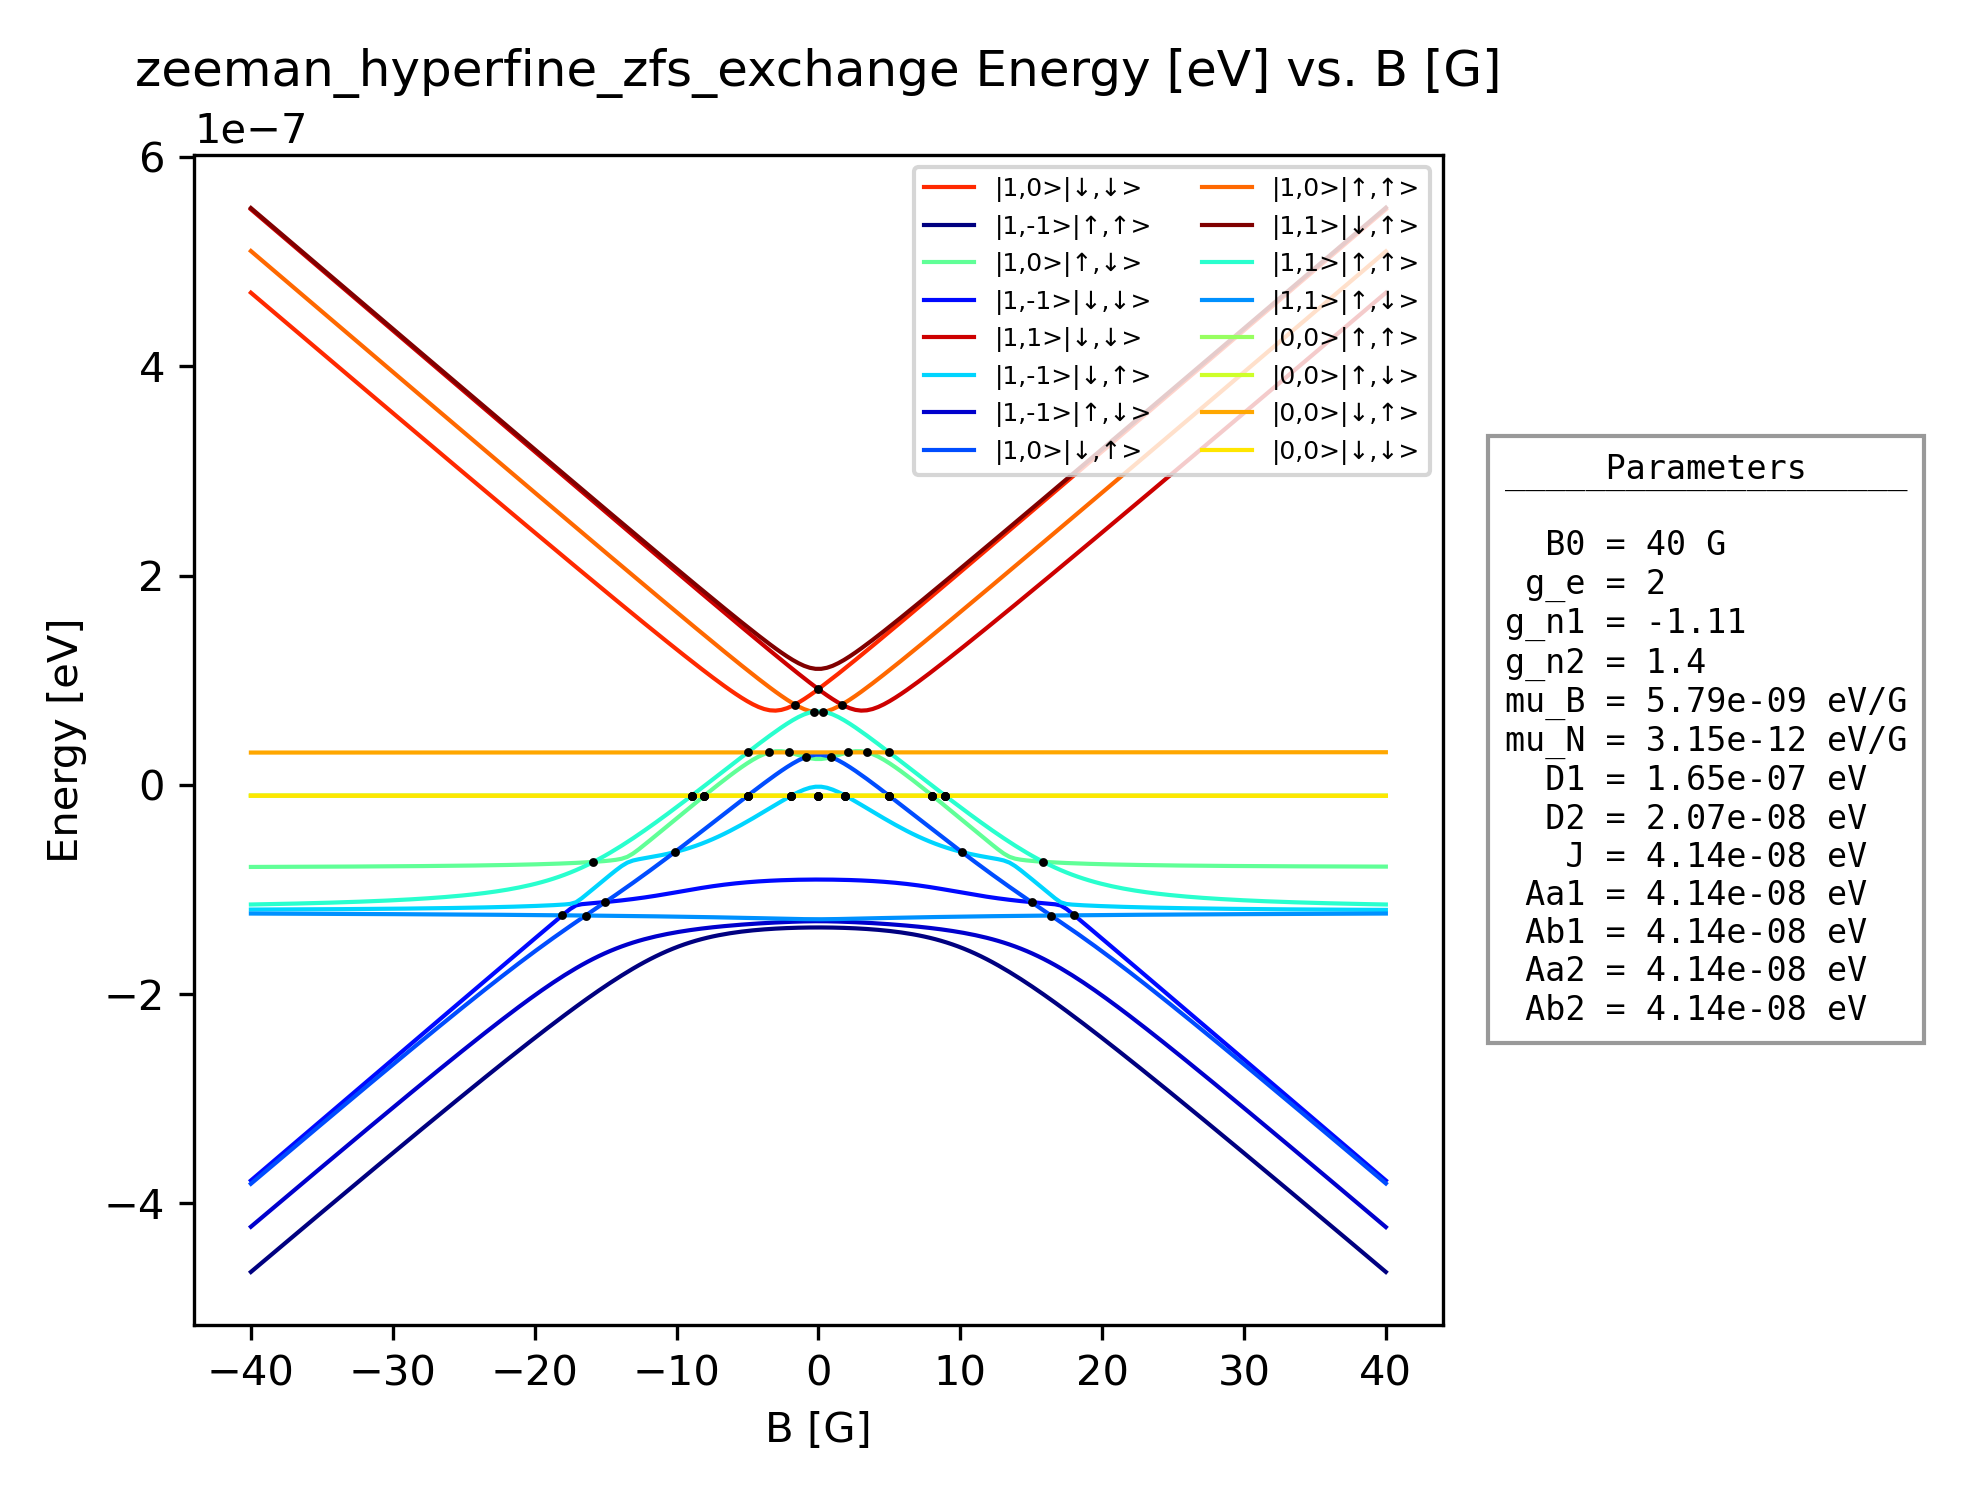
\includegraphics[width=11cm]{full.png}
  \caption{Eigenenergies of the full $16\times16$ Hamiltonian across $\pm40$\,G. Highlighted points mark relevant degeneracies.}
  \label{fig:eigenspectra}
\end{figure}

For full implementation details see the online manuscript.\footnote{https://dev-undergrad.dev/posts/spin\_hamiltonian\_simulation/}

% =============================================================
\section{Solving the Stochastic Liouville Equation}\label{sec:sle}
% =============================================================
To model the \mbox{non\hyp{}equilibrium} spin dynamics we solve the steady\hyp{}state Stochastic Liouville Equation (SLE)
\[
  0 = -\frac{i}{\hbar}[\hat{H}_0,\rho] - \frac{k}{2}\{\Lambda,\rho\} + p\,\Gamma,
\]
where $\rho(B)$ is the $16\times16$ density matrix. Recasting into Sylvester form yields
\[
  A\,\rho + \rho\,A^{\dagger} + g = 0,
\]
with
\[
  A = -\frac{i}{\hbar}\hat{H}_0 - \frac{k_S+k_D}{2}\,\Lambda_S - \frac{k_D}{2}\,\Lambda_T,\qquad
  g = -\frac{p}{16}\,\Gamma.
\]
Vectorising that expression produces a $256\times256$ linear system, which we solve numerically for each field value to obtain $\rho(B)$; details are given online.\footnote{https://dev-undergrad.dev/posts/sle/}

% =============================================================
\section{Simulating EDMR}\label{sec:edmr}
% =============================================================
The full \emph{time\hyp{}dependent} Hamiltonian relevant to an EDMR experiment reads
\[
  \mathcal H(t)=\hat{H}_0 + \hat{H}_{\mathrm{HF,sec}} + \hat{H}_{\mathrm{MW}}(t),
\]
with
\[
  \hat{H}_{\mathrm{HF,sec}} = \sum_{i=1}^{2} \hat{\mathbf S}\cdot \hat{A}_{iz}\cdot \hat{\mathbf I}_i,
  \qquad
  \hat{H}_{\mathrm{MW}}(t)=\frac{h\omega_1}{2}S_x\!\left(e^{i2\pi\nu t}+e^{-i2\pi\nu t}\right).
\]
Performing the Rotating Wave Approximation (RWA) discards the \mbox{fast\hyp{}oscillating} counter\hyp{}rotating term, leaving the \mbox{time\hyp{}independent} effective Hamiltonian
\[
  \mathcal H^{\pm} = \hat{H}_0 - G \pm \frac{h\omega_1}{2}S_x,
  \quad
  G = h\nu S_z + \hat{H}_{\mathrm{HF,sec}}.
\]
The $+$ sign retains the \mbox{co\hyp{}rotating} component that drives transitions. Solving the steady\hyp{}state SLE with $\mathcal H^{+}$ yields the density matrix $\rho(B)$, from which the \emph{singlet population}
\[
  I(B)=A\,\mathrm{Tr}\!\bigl(\Lambda_S\rho(B)\bigr)+I_0
\]
is directly proportional to the measured current.

\begin{figure}[H]
  \centering
  
\includegraphics[width=\linewidth]{EDMRLSQ.png}
  \caption{Simulated EDMR model fitted against experimental data taken at 2\,G peak\hyp{}to\hyp{}peak modulation, 200\,MHz RF, and 3.5\,V bias.}
  \label{fig:edmr_lsq}
\end{figure}

\newpage
% =============================================================
\section{References}
% =============================================================
\noindent
My own documents: \\ 
\texttt{https://dev-undergrad.dev/posts/spin\_hamiltonian\_derivation/}  \\
\texttt{https://dev-undergrad.dev/posts/spin\_hamiltonian\_code/}  \\
\texttt{https://dev-undergrad.dev/posts/spin\_hamiltonian\_simulation/}  \\
\texttt{https://dev-undergrad.dev/posts/sle/}  \\

\medskip\noindent
Christopher Tao-Kuan Lew. \emph{All-Electrical Quantum Sensing with Silicon Carbide Devices}. PhD thesis, University of Melbourne, June 2022. ORCID 0000-0001-6432-4520.  

\medskip\noindent
Elias B. Frantz. \emph{Development of the Analytic Capabilities of Near-Zero Field Magnetoresistance Spectroscopy Through Experiment and Modeling of the Stochastic Quantum Liouville Equation}. PhD dissertation, The Graduate School, The Pennsylvania State University, 2021.  

\medskip\noindent
Kazuyuki Fujii. \emph{Introduction to the Rotating Wave Approximation (RWA): Two Coherent Oscillations}. arXiv:1301.3585 [quant-ph], 23 May 2014.  

\end{document}

